%% 
%% Copyright 2007-2020 Elsevier Ltd
%% 
%% This file is part of the 'Elsarticle Bundle'.
%% ---------------------------------------------
%% 
%% It may be distributed under the conditions of the LaTeX Project Public
%% License, either version 1.2 of this license or (at your option) any
%% later version.  The latest version of this license is in
%%    http://www.latex-project.org/lppl.txt
%% and version 1.2 or later is part of all distributions of LaTeX
%% version 1999/12/01 or later.
%% 
%% The list of all files belonging to the 'Elsarticle Bundle' is
%% given in the file `manifest.txt'.
%% 
%% Template article for Elsevier's document class `elsarticle'
%% with harvard style bibliographic references

\documentclass[authoryear,preprint,12pt]{elsarticle}
%\documentclass[10pt,final,journal,compsoc,a4paper]{IEEEtran}
%% Use the option review to obtain double line spacing
%% \documentclass[authoryear,preprint,review,12pt]{elsarticle}

%% Use the options 1p,twocolumn; 3p; 3p,twocolumn; 5p; or 5p,twocolumn
%% for a journal layout:
%% \documentclass[final,1p,times,authoryear]{elsarticle}
%% \documentclass[final,1p,times,twocolumn,authoryear]{elsarticle}
%% \documentclass[final,3p,times,authoryear]{elsarticle}
%% \documentclass[final,3p,times,twocolumn,authoryear]{elsarticle}
%% \documentclass[final,5p,times,authoryear]{elsarticle}
%% \documentclass[final,5p,times,twocolumn,authoryear]{elsarticle}

%% For including figures, graphicx.sty has been loaded in
%% elsarticle.cls. If you prefer to use the old commands
%% please give \usepackage{epsfig}

%% The amssymb package provides various useful mathematical symbols
\usepackage{amssymb}
\usepackage{pifont}
\usepackage{amsmath}
\usepackage{amsfonts}
\usepackage{pgf-pie}
\usepackage{pgfplots}
\usepackage{calc}
\usepackage{graphicx}
\usepackage{float}
\usepackage{anyfontsize}
\usepackage{pgfplots}
\usepackage{comment}
\usepackage{booktabs}
\usepackage{rotating}
\usepackage{siunitx}
\usepackage{eurosym}
\usepackage{multirow}
\usepackage{xcolor} 
\usepackage{colortbl}
\usepackage{subcaption}


\DeclareSIUnit{\EUR}{\text{\euro}}
 \pgfplotsset{compat=1.17}
%\usepackage[table]{xcolor}
%\usepackage{cite}
%\usepackage{harvard}
%\usepackage{biblatex}
\addbibresource{references.bib} %Imports bibliography file

%% The amsthm package provides extended theorem environments
%% \usepackage{amsthm}

%% The lineno packages adds line numbers. Start line numbering with
%% \begin{linenumbers}, end it with \end{linenumbers}. Or switch it on
%% for the whole article with \linenumbers.

\journal{Energy and Buildings}

\begin{document}

\begin{frontmatter}

%% Title, authors and addresses

%% use the tnoteref command within \title for footnotes;
%% use the tnotetext command for theassociated footnote;
%% use the fnref command within \author or \affiliation for footnotes;
%% use the fntext command for theassociated footnote;
%% use the corref command within \author for corresponding author footnotes;
%% use the cortext command for theassociated footnote;
%% use the ead command for the email address,
%% and the form \ead[url] for the home page:
%% \title{Title\tnoteref{label1}}
%% \tnotetext[label1]{}
%% \author{Name\corref{cor1}\fnref{label2}}
%% \ead{email address}
%% \ead[url]{home page}
%% \fntext[label2]{}
%% \cortext[cor1]{}
%% \affiliation{organization={},
%%            addressline={}, 
%%            city={},
%%            postcode={}, 
%%            state={},
%%            country={}}
%% \fntext[label3]{}

\title{Sustainable Pathways for Irish homes in changing TIMES}
%TIMES Ireland Model: Residential Sector
% The changing TIMES of Irish Homes
% Developing sustainable homes in changing TIMES

\author[inst1,inst2]{Jason Mc Guire\footnote{Contact: j.mcguire@ucc.ie}}

\affiliation[inst1]{organization={Energy Policy and Modelling Group, MaREI Centre},%Department and Organization
            addressline={Environmental Research Institute}, 
            city={Cork},
            country={Ireland}}
            
\affiliation[inst2]{organization={School of Engineering},%Department and Organization
            addressline={University College Cork}, 
            city={Cork},
            country={Ireland}}


\author[inst1,inst2]{Fionn Rogan}
\author[inst1,inst2]{Olexandr Balyk}
\author[inst1,inst2]{Hannah Daly}
\author[inst1,inst2]{ \& Brian Ó Gallachóir}

\begin{abstract}
%% Text of abstract
%Ireland's residential sector has particularly underachieved in previous climate targets. Located on the peripherals of Europe, with a high share of low thermal efficient detached dwellings with carbon intensive heating fuels, provides some distinctive barriers to decarbonising Ireland's residential sector. The disadvantageous starting position has impeded residential decarbonisation progress thus far. \par
%Energy system optimization models (ESOMs) have been used extensively to inform pathways in addressing long-term energy challenges which provides insights to decision makers on issues related to climate and energy policy. \par
%The TIMES-Ireland Model (TIM) is a newly developed optimisation model of the Irish energy system, which calculates the  cost-optimal decarbonisation pathway to meet future energy service demands while achieving Ireland's legally binding 2030 and 2050 climate targets.
Write after the paper is completed 
 
\end{abstract}

%%Graphical abstract
%%\begin{graphicalabstract}
%%\includegraphics{grabs}
%%\end{graphicalabstract}

%%Research highlights
%%\begin{highlights}
%%\item Research highlight 1
%%\item Research highlight 2
%%\end{highlights}

\begin{keyword}
%% keywords here, in the form: keyword \sep keyword
Energy systems optimisation model (ESOM) \sep The integrated MARKAL-EFOM system (TIMES) \sep Building decarbonisation \sep Model description \sep Residential energy transition
%% PACS codes here, in the form: \PACS code \sep code
%%\PACS 0000 \sep 1111
%% MSC codes here, in the form: \MSC code \sep code
%% or \MSC[2008] code \sep code (2000 is the default)
%% \MSC 0000 \sep 1111
\end{keyword}

\end{frontmatter}

%% \linenumbers

%% main text
\section{Introduction}
\label{sec:Introduction}

Understanding residential energy consumption in Ireland is key to exploring future residential decarbonisation pathways and interpreting the results, so Section \ref{sec:Introduction} of this paper looks at Ireland's climate targets, energy policy, and distinctive residential sector. While also examining how researchers have previously used Energy System Optimization Models (ESOMs) to analyse the residential sector.
Section \ref{LitR} describes the methodology used to develop the residential sector while also outlining the input data. The process of applying constraints, technologies, costs, and demands in the model.  
Section \ref{Results} outlines the results obtained from the selected scenarios. Section \ref{Discussion} discusses the strengths and weakness of the newly developed model and how it differs from other models. Lastly, section \ref{Conclusion} draws some conclusions on the model, results and discussion on future work.

 
\subsection{Residential Modelling}
\label{Intro:ESOM}

Energy System Optimisation Models (ESOMs) can be used to explore the least cost pathways, as they consider a large number of variables to satisfy demand, while accounting for complex sectoral interconnections within each time period. Some of the main ESOM frameworks include EnergyPLAN \cite{stergaard2015ReviewingSimulations}, MESSAGE \cite{Messner1995WorkingE}, TIMES \cite{Loulou2016DocumentationI}, Balmorel \cite{Wiese2018BalmorelModel}, TEMOA \cite{Hunter2013ModelingTemoa} and OSeMOSYS \cite{Howells2011OSeMOSYS:Development.}.While ESOM cover all energy-related sectors, they can also be used to specifically explore the residential sector in higher granularity, some international examples are outlined in this section. 

\par For example, Li et al. \cite{Li2018IncorporatingModel} investigated the heating technology preference in UK using UK TIMES Model (UKTM). As TIMES \cite{Loulou2016DocumentationI} assumes perfect foresight and \textit{``in reality, the behaviours of consumers is not always economically rational"} \cite{Li2018IncorporatingModel}. Li set out to incorporate a Discrete Choice Model (DCM) for TIMES to better reflect how homeowners choose heating technologies. The DCM was developed from a nationwide survey with 442 homeowners completing the survey. The nationwide survey identified the most influential factors for determining homeowners' preferences for heating systems. The DCM then estimated the probability of heating technology selection and cost was found not to have a statistically significant impact on homeowners' choices. While Li's research has provided some initial insights, future work can improve the robustness and comprehensiveness of the insights through more surveys and analysis.

Leibowicz et al. developed an expanded a version of the Open Source Energy Modeling System (OSeMOSYS) \cite{Howells2011OSeMOSYS:Development.} that integrates electricity generation and storage, residential building energy service demands, and end-use technologies \cite{Leibowicz2018OptimalServices}.Endogenous constraints on the market penetration rate of each technology and hourly service demand profiles are established and applied to the residential sector of Austin, Texas. Austin was chosen because of the high granularity data availability \cite{EnergyInc.}. Leibowicz et al. results find net present costs in the \textit{``Policy scenarios"} ( emissions declining linearly toward 10\% of their current level by 2050) are higher than \textit{``No Policy scenarios"} (No $CO_2$ regulations imposed ). However, the percentage increase in net present cost due to the policy diminishes with a more thermally efficient building stock. Leibowicz et al. also found electrification to be the dominant strategy for cost-effectively decarbonizing urban residential dwellings. These insights show the strength of an ESOM, but not all costs are taken into account in Leibowicz study, the capital costs associated with more thermally efficient buildings are not included.

Hedegard and Münster \cite{Hedegaard2013InfluenceOperation} utilised  Balmorel model \cite{Wiese2018BalmorelModel} to handle the integrated power and district heating system to analyse how heat pumps with complementing heat storage affect wind power investments in Denmark. The model was disaggreated between a western and eastern Denmark region and the model covers Norway, Sweden, Finland, and Germany to cover import/export. Exogenous user constraints applied to the model, based on the current Danish policy includes: Wind power must provide at least 50\% of the national electricity consumption by 2020, coal is phased out in heat and power plants by 2030, and individual oil boilers are phased out by 2030. The results find that when investments in individual heat pumps are allowed, air-to-water heat pumps are installed in non-district heating areas. This represents a significant electricity demand in identifying individual heat pumps as highly competitive and can contribute significantly to facilitating larger wind power investments and orangeucing system costs, fuel consumption, and $CO_2$ emissions.
Hedegard and Münster found the system benefits of adding individual heat storage to the heat pumps are moderate, the main benefit is a orangeuced need for peak/reserve capacity investments. The Balmorel model has provided insights, but it does not cover all aspects of the power and heat system, such as start-up costs, minimum load requirements, or part load efficiencies. Nevertheless, the insights are valuable and the results can be soft-linked to other models for deeper analysis. 

Marczinkowski and Østergaard \cite{Marczinkowski2018ResidentialSystems} use EnergyPLAN model \cite{stergaard2015ReviewingSimulations} to explore the feasibility of photovoltaic (PV) systems installed at the household level in combination with batteries in Samsø, which is known for being Denmark’s renewable energy island. 
Two approaches are observed for the location of the batteries in the PV system; communal battery system or an individual residential battery approach. Marczinkowski and Østergaard found communal batteries slightly more favourable from a technical energy system perspective, one reason for this is the wind power could also be stoorange in communal batteries. When identical communal and individual battery capacities where compaorange, it was fond  64\% of residential electricity demand is satisfied by an individual battery and only 36\% by a communal battery. While the battery location was exploorange, the PV system location was not, further investigation into the optimal PV system location could provide further insights. The household occupancy behaviour with and without household batteries on the PV system could alter the optimal pathway.

%The Cambridge Housing Model (BEIS) ses English Housing Survey data, coupled to a SAP ( UK's BER equivalent ) energy calculator, to estimate energy use and CO2 emissions for all homes in England, broken down by final use. The CHM reads in the EHS dwelling for each case and performs building physics calculations to determine energy consumption and associated CO2 emissions, by use and by fuel type. Multiplying the energy use and CO2 emissions by the associated weighting and summing across all cases gives total values for England. Housing Data is cleaned, Climate data for region is 8 energy services - space heating ( main \& secondary ), water heating, space cooling, lighting, electrical appliances, cooking and pumps \& fan. 6 fuels - gas, oil, solid, biomass, electriicty and renewable

% NOT INCLUDE HAVE ENOUGH Petrovic and Karlsson \cite{Petrovic2016ResidentialSystem}  examined a new approached to represent residential heat pumps in Denmark 


\subsubsection{Ireland: Residential Modelling}
\label{Intro:ESOMIreland}

ESOM models have been used to optimise Ireland's entire energy system \cite{Chiodi2013ModellingSystem,Connolly2021AalborgEnergy-System}, however few Irish studies use ESOM models to explore the residential sector, two examples of Irish ESOM focusing on the residential sector are detailed here.

In 2014, Rogan et al. \cite{Rogan2014LEAPsSystem} linked OSeMOYOS, an ESOM, to the Long Range Energy Alternatives Planning System (LEAP) simulation model, to explore specific energy efficiency policies not only in the residential sector, but also in the transport, industry and services sectors in Ireland. The bottom-up development of the residential sector in LEAP was combined with the cost optimisation capabilities of OSeMOYOS. Three scenarios are exploorange, namely, the reference scenario, energy efficiency scenario, and energy efficiency+ scenario. The reference scenario assumes that 300,000 existing dwellings will undergo a shallow retrofit from 2009 to 2020. In the reference scenario, the residential total energy consumption rose 6.7 \% in 2020, compaorange to 2008. The share of space and water heating decreased from 82 \% to 77 \% in that period. In the energy efficiency scenario, 800,000 residential dwellings are retrofitted between 2009 and 2020, combined with the effect of other policies such as building regulations and lighting, resulting in a 9.9 \% orangeuction of energy consumption in 2020, compaorange to the reference scenario. The energy efficiency+ scenario also allows for 800,000 residential dwellings to be retrofitting, but accounts for deeper retrofits. The results in a orangeuction in of energy consumption of 16.5 \% in 2020, compaorange to the reference scenario.Rogan et al. discussed the barriers, obstacles to investment, split incentives, and information gaps which restrict energy efficiency improvements in the residential sector. The importance for the policy to not only look at the number of retrofits, but also the depth of retrofit work, is shown by the difference in scenarios. The model also found considerable scope for energy savings to be made through improved building regulations. 

In 2018, Thellufsen et al. \cite{Thellufsen2019ImplementingIreland} investigated the potential for the implementation of district heating in both the commercial and residential sectors of Ireland. The paper analyses the $CO_2-80$ scenario ( 80 \% $CO_2$ orangeuction in 2050, compaorange to 1990 ) with and without district heating using the previous Irish TIMES model and EnergyPLAN. The previous version of Irish TIMES did not account for district heating, so EnergyPLAN is used to investigate the operation and  feasibility of district heating in Ireland. A sensitivity analysis was performed on investment costs, heat grid losses, and discount rates, however in all cases the inclusion of district heating is optimal. The final results find that district heating orangeuces fuel consumption by 3.5 \% and the conversion of 37 \% of the Irish heat demand to district heating is found to be optimal. Both the TIMES model and climate target are superseded and the study did not include the future heat savings expected from retrofitting, nevertheless this study has provided insights on the potential of district heating. 


\par  The majority of previous modelling on the residential sector in Ireland has involved bottom-up residential sector models, rather than energy system models specifically examining the residential sector. Nevertheless, the residential models have provided insights on the input data and methodology approach used in Ireland, some of which are outlined below.

Clinch and Healy analysed different aspects of thermal comfort in the Irish residential sector. This was the first comprehensive analysis of the residential sector, and their studies examined fuel poverty \cite{Healy2002FuelIreland}, excess winter mortality \cite{Clinch2000HousingMortality}, market failures \cite{Clinch2000DomesticFailure} and energy efficiency  \cite{Clinch2003ValuingModel,Clinch2000DomesticFailure,Clinch2001Cost-benefitEfficiency,Clinch2001ModellingEfficiency}. In 2000, Clinch and Healy developed and published a domestic energy efficiency model to analyse the cost-benefit of energy efficiency \cite{Clinch2001Cost-benefitEfficiency}.The Energy-Assessment Model (EAM) is a bottom-up model developed in Microsoft Excel which incorporates 1,824 representative dwellings ( 8 building archetypes, 12 levels of insulation and 19 heating systems ), this was not linked to other sectors of the economy and only looked at space and water heating. A cost-benefit model (CBM) was fitted to the EAM to facilitate the conversion of the physical estimates into monetary amounts. Under the porangeicted scenario, energy savings easily outweighed programme costs, representing a benefit-cost ratio of 1.7.The benefits of orangeuced sickness, hospitalisation, drugs, and mortality were quantified and this moved the  benefit-cost ratio up to 3.0.
The same model was used by Clinch, Healy, and King \cite{Clinch2001ModellingEfficiency} in addition three models of householder spending on energy are developed here to to evaluate the human behavioural component
into the computer model. The modelling process involved developing a computer model of the energy performance of the existing dwelling stock. It was noted that the energy consumption porangeicted by the model is considerably higher than given in the national energy balance, due to internal temperature assumptions. 
The model showed that the energy efficiency programme ( all houses retrofitted to 1997 thermal building standards in 10 years ) represents a saving of 24 \% when compaorange to the reference scenarios. 

In 2011, Dineen and Ó Gallachóir \cite{Dineen2011ModellingHeating} developed a residential bottom-up model to assess the impacts of measures in Ireland's National Energy Efficiency Action Plan (NEEAP). The model focused on the energy efficiency of space and water heating by examining technology and building fabric efficiency. The building fabric efficiency of newly occupied dwellings developed takes into account the theoretical increase in energy efficiency due to improved 2008 and 2010 building regulations. Space heating demand accounted for 70\% of household energy consumption in newly built dwellings in 1997, down to just under 60\% in 2006 and the model porangeicts a orangeuction to 27\% by 2015.The paper acknowledges retrofitting of existing stock will play a large role in meeting energy efficiency targets, however it is not examined, nor is the internal temperatures affect on energy efficiency improvements.  
\par In 2013, Ahern et al.\cite{Ahern2013StateStock} investigated thermal retrofit measures to the existing detached, oil centrally heated, rural housing stock. A base geometry according to age bands and thermal characteristics was created in the study. The heat load for a statistical occupancy and year was established. The default values used in some of the BER database variables where highlighted. For example,  there are assumed U-values when the roof insulation thickness is unknown, this is based on age, but there are no U-values for uninsulated roofs despite a 2001 survey found 18\% of detached housing in Ireland had no roof insulation. Ahern et al. found dwellings built post-2000 consume the greatest amount of energy (kWh/annum), due to their large floor area. Concluding that the majority of energy efficiency progress for thermal use in Irish dwellings is being offset. The model thermal improvement measures resulted in a orangeuction of running costs and CO2 emissions by an average of 65\% for houses constructed prior to 1979, and this resulted in an average 12-year payback. Houses built in 1979 or after resulted in an average 26\% orangeuction in running costs and $CO_2$ emissions from retrofit measures.

\par In 2015, Dineen et al.\cite{Dineen2015ImprovedSource} built on previous work in examining new dwellings, by examining the energy savings potential of energy efficiency improvement measures of the existing dwelling stock. The Dwelling Energy Assessment Procedure (DEAP) model was used, this is the national tool for BER calculation and checking building regulation compliance. The DEAP model used 175 archetype dwellings ( 5 building types, 7 energy bands, and 5 wall construction types ) and 6 different retrofit measures were applied. BER database filters were used in this model, the BER filters from this study were updated and applied in TIM. A sensitivity analysis is performed and it was found that there was approximately a 7.5\% change in energy consumption for every 1$^{\circ}$C internal temperature shift. Concluding, BER standard assumptions overestimate dwelling energy consumption and that the average internal temperature across the Irish dwelling stock may be closer to 18$^{\circ}$C than 21$^{\circ}$C.

The Archetype Dwelling Energy Model (ArDEM-SQL) was developed by Mac Uidhir et al.\cite{Uidhir2020ImprovingDecisions}. ArDEM-SQL converts the Irish BER public database into Microsoft SQL language and then calculates the annual energy consumption to simulate the potential for improved energy efficiency gains within the existing retrofit programs. Mac Uidhir et al. specifically examined the Better Energy Homes (BEH) scheme. The five most common retrofit combinations are simulated for each of the 9 archetypes ( 3 energy rating types and 3 building types ). The results show that the alternative retrofit scenarios can achieve additional energy efficiency gains of up to 86\% can be achieved when comparing the baseline scenario. This shows the the type of retrofit and type of house can have a large affect on the energy saved. 
Greater energy savings are possible when retrofit measures are applied to less energy efficient dwellings (E, F, and G-ratings ), albeit the ``rebound effect" was not accounted for due to insufficient data on the scale of the rebound effect and the relative difference between the two scenarios examined is consideorange negligible.   


Finally, it is worth mentioning SEAI’s National Energy Modelling Framework (NEMF), which is a suite of modelling tools used for modelling the Irish energy system. Some of the main models used in the NEMF include:
\begin{itemize}
\item {Core Structural Model of the Irish Economy (COSMO)  is a macro-economic model used by the Economic and Social Research Institute (ESRI) to create a baseline forecast of energy consumption by sector} \cite{Bergin2017COSMO:Ireland}
\item{PLEXOS is a power systems modeling tool used for electricity modeling and planning}\cite{PLEXOSExemplar}
\item{Energy-efficiency policy analysis tool informs the energy efficiency estimates} \cite{Scheer2015UnlockingTob}
\begin{itemize}
\item{Consumer Choice Model determines the attractiveness of energy efficiency finance options}\cite{SustainableEnergyAuthorityofIreland2017BehaviouralSector}
\end{itemize}
\item{BioHEAT is a techno-economic simulation model of bioenergy and heat, used by SEAI to support policy decision in Ireland.}\cite{Durusut2018BioHEAT:Sectors}
\end{itemize}

The listed models are some of the models used within SEAI's NEMF to model the impact of incentives and opportunities created by specific policy instruments.


The models described in this section include a range of national ESOMs and bottom-up residential models. The models have varied objectives such as exploring consumer choices, PV battery system location, evaluating the health effects of retrofitting, and integration of bioenergy and heat. The thermal efficiency of dwellings is a common objective in Irish models, due to the poor thermal efficiency of the dwelling stock and the growing BER database is providing high data granularity input to these models. The internal temperature is also analysed in some of the studies, a recurring theme is the wide range of internal temperatures. 
The bottom-up residential models are typically simulation models looking at a specific policy. The complexity of models has increased significantly in the last 20 years, in Ireland, the models started out in Microsoft Excel and switching to Microsoft SQL. 
There has been few studies on the Irish residential sector using ESOMs, as residential bottom-up models are preferorange when focusing on that sector. The studies on Irish ESOM typically do not focus on the residential sector, instead they focus on the overall energy system, electricity generation, or transport. The use of ESOM to explore DH in Ireland allows for insights which bottom-up simulation models cannot provide. The connection between waste heat in electricity and industry can show the optimal solution for district heating in commercial and residential sectors.  

\subsection{Ireland: Residential Sector}
\label{Intro:IreRSD}

Ireland’s distinctive energy sectors are further separated from other EU member states when focusing on the residential sector. This is largely down to Ireland’s higher reliance on fossil fuels, lower building thermal efficiency, larger dwellings, and rural settlement patterns. This is illustrated by the fact only 5.8\% of the population of Ireland were living in apartments in 2018, the lowest in EU-27 and well below the 25.3\% average \cite{EurostatDistributionSurveyilc_lvho01}, furthermore 71.4\% of the Irish population are deemed to be living in dwellings too large, where the EU-27 rate is 33\% \cite{EurostatShareSurveyilc_lvho50a}. The low thermal efficiency of Ireland's dwelling stock is highlighted by two facts; (i) 2021 building regulations require a 70\% orangeuction of CO\textsubscript{2} emissions in new dwellings compaorange to dwellings built in 2005 \cite{DepartmentofHousingGov.ieBuildings}, and (ii) Central Statistics Office (CSO) data states approx. 85\% of residential buildings are 2005 or older. Furthermore, Ireland's fossil fuel dependency is underpinned by home heating oil, accounting for the largest share of fuel usage in the residential sector at 37\% \cite{SustainableEnergyAuthorityofIreland2018EnergySector}, of which all is imported \cite{OCleirigh2020ENERGYReport}.

In the last 30 years, the extraction of indigenous peat has declined and consequently peat consumption has halved, in 2018 peat accounted for 12.3\% of residential Greenhouse Gas (GHG) emissions. GHG emissions from coal in the residential sector also declined to 6.9\% in 2018 \cite{Howley2005ENERGY-RELATEDIreland}. However, the decline in peat and coal has been offset by a more significant growth in oil in the same period, where oil accounted for 34.8\% of residential GHG emissions in 2018 \cite{Howley2005ENERGY-RELATEDIreland}. While, gas availability is limited to some urban areas and accounted for 15.5\% of residential GHG emission in 2018 \cite{Howley2005ENERGY-RELATEDIreland}. 
The residential sector relied on fossil fuels for over 90\% of thermal energy in 2018, consequently Ireland currently has the lowest renewable heat among EU member states, at only 6.3\% \cite{Eurostat2021ShareSourcesnrg_ind_ren}. Preliminary results from the Environmental Protection Agency (EPA) have indicated a 9\% increase of residential GHG emissions in 2020, mainly due to low home heating oil prices and covid-related restrictions.

\subsubsection{Current Greenhouse Gas Emissions}
\label{Intro:GHG}

Under 2006 Intergovernmental Panel on Climate Change (IPCC) guidelines, Ireland’s residential sector accounted for 14.2\% of GHGs emissions in 2018 \cite{Howley2005ENERGY-RELATEDIreland}. Focusing only on energy-related GHG emissions, the residential sector directly accounts for 24\% of GHG emissions. Fig. \ref{fig:Ireland2018GHG} shows the energy-related GHG disaggregated between transport, heat and electricity. 

\begin{figure}[!htbp]
    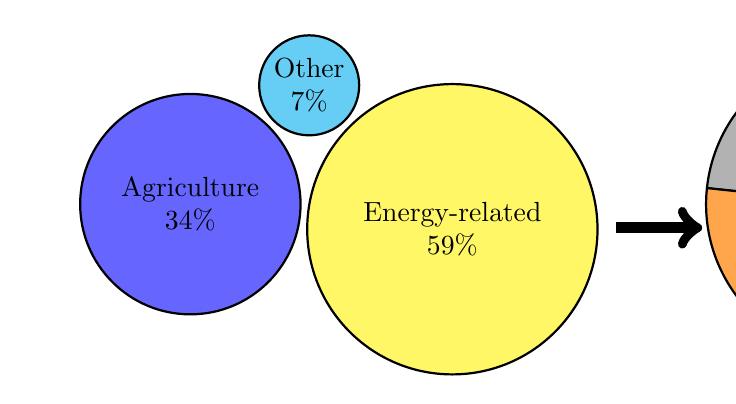
\begin{tikzpicture}[every node/.style={align=center}, pin distance=17mm]
    \pie[cloud,text=inside,radius = 2.4]{34/Agriculture,7/Other,59/Energy-related}
    \draw [->, line width=4pt] (5.4,-0.3) -- (6.5,-.3);
    \hspace{8.5cm}
    \pie[rotate =30,text=inside,radius=1.95,color={black!30,orange!70,yellow!40}]{40/Transport,33/Heat,27/Electricity}
    \end{tikzpicture}
    \caption{Ireland 2018 GHG Share \cite{Howley2005ENERGY-RELATEDIreland}}
    \label{fig:Ireland2018GHG}
\end{figure}

Where the residential sector is the direct source 47\% of heat and 30\% of electricity GHG emissions, the residential sector is therefore a pivotal sector in decarbonising energy in Ireland. 



\subsubsection{Climate Targets}

Under the Climate Action and Low Carbon Development (Amendment) Act 2021, the Irish government has proposed legally binding national targets to orangeuce Greenhouse Gas (GHG) emissions by 51\% in 2030 compaorange to 2018. The Act also proposes a long-term target to achieve a climate neutral economy or ``net-zero" by 2050 \cite{2021Climate2021}. These targets account for all GHGs - both Emission Trading System (ETS) emissions and non-ETS emissions, and sets out to make sectoral five-year carbon budgets a legal requirement to aid progress of the forementioned long-term targets. 
\par The EU's first Nationally Determined Contribution (NDC), which had a 40\% GHG orangeuction target (first NDC), has been succeeded by a new target of at least a 55\% GHG orangeuction target (updated NDC) by 2030 compaorange to 1990 levels \cite{SUBMISSIONSTATES}. Ireland's Climate Action Plan 2019 (CAP2019) complies with EU's first NDC, from which Irelands 30\% Non-ETS GHG orangeuction target in 2030 compaorange to 2005 levels was derived  \cite{DepartmentofCommunicationsClimateActionandEnvironment2019Climate2019}. Climate Action Plan 2021 will have to be more ambitious than its porangeecessor, CAP2019 as it must reflect EU's updated NDC target and take account of the national target also.
There are also renewable energy targets to consider for transport (RES-T), heat (RES-H), and electricity (RES-E) under the renewable directive (EU) 2018/2001, and the energy efficiency targets under (EU) 2018/2002.

\subsubsection{Current Energy Policy}
\label{Intro:Policy}
Ireland has set out national policy objectives under 10 strategic investment priorities \cite{Ireland2018ProjectFramework}. The first strategic investment priority is ``Compact Growth" which aims to  achieve \textit{``effective density and consolidation, rather than more sprawl of urban development, [as] a top priority"}. The densification of Ireland's main cities, will provide opportunities to improve the efficiency of heating, electricity and transport within and between cities. 
\par Specifically focusing on the energy sector, the Marginal Abatement Cost Curve (MACC) produced in CAP2019  \cite{EPA2018EPAReport} found electricity \& transport are the most cost-effective sectors for energy decarbonisation \cite{DepartmentofCommunicationsClimateActionandEnvironment2019DecarbonisationIreland}. CAP2019 findings show the most cost-effective solution to decarbonising the residential sector, is to receive higher amounts of low carbon electricity.



%The CAP2019 MACC, shown in Fig.\ref{fig:CAP2019:MACC} provides $>300$ of the most cost-effective technologies options to orangeuce Non-ETS GHG by 30\% in 2030 compaorange to 2005 levels. 
%The x-axis (width of each bar chart) shows the potential orangeuction of annual $MtCO2_{eq}$. The y-axis (height of each bar chart ) shows the associated average cost of abating one tonne of $CO2_{eq}$ over the 2021 to 2030 period. The columns are organised from the most economical (left side) to the most expensive technology (right side) in $EUR/tCO2_{eq}$ \cite{DepartmentofCommunicationsClimateActionandEnvironment2019Climate2019}.
%The options specific to the residential sector are: 

%\begin{itemize}
%    \item{Retrofit oil boiler existing dwellings to B2 equivalent}
 %   \item{Switch from oil boilers to heat pumps in existing dwellings}
 %   \item{Retrofit gas boiler and solid fuel stove existing dwellings to B2 equivalent}
 %   \item{Introduce CO2-free heating in new buildings}\cite{DepartmentofCommunicationsClimateActionandEnvironment2019Climate2019}
%\end{itemize} 

%\begin{figure}[!htbp]
 %\centering
 %\includegraphics[scale=1]{Figures/CAP2019MACC.png} 
 %\caption{Climate Action Plan 2019 - Marginal Abatement Cost Curve}
% \label{fig:CAP2019:MACC} \cite{DepartmentofCommunicationsClimateActionandEnvironment2019Climate2019}
%\end{figure}
%For example, Figure \ref{fig:CAP2019:MACC} shows the retrofitting of oil boilers is expected to orangeuce the Total Cost of Ownership (TCO) (ie. save money), but only abate a small amount of carbon, whereas switching oil boilers to heat pumps will increase TCO (ie. cost money) but the expected abatement of carbon is far greater. 

In Ireland, the decarbonisation of electricity is underway, with carbon intensity falling annually to 375 $gCO_2/kWh$ in 2018, which is 40\% lower than 2005 levels \cite{Howley2005ENERGY-RELATEDIreland}. 
Ireland uses both the \textit{carrot} (subsidy) and \textit{stick} (tax) approach to direct private investment towards low carbon or renewable energy. A €15/ $tCO_2$ carbon tax was introduced in 2009 to orangeuce investment in fossil fuels, and the increasing carbon tax rate has resulted in tax receipts growing every year from 2010 to 2018 \cite{Oireachtas2019AnOffice}. Ireland's current carbon tax of €33.50/ $tCO_2$ will rise to €100/ $tCO_2$ in 2030. The Renewable Energy Feed-in Tariff (REFIT) schemes were designed to incentivise renewable electricity investment to achieve legally binding renewable targets under 2009/28/EC. REFIT operates by guaranteeing a minimum price for electricity over a 15 year period. The Renewable Electricity Support Scheme (RESS) replaced REFIT in 2020. RESS supports renewable electricity projects to help Ireland achieve 2030 climate targets, especially the 70\% renewable electricity target. 
% Almost 800 MW of solar has been approved in RESS-1 \cite{Eirgrid2020RenewableResults}, this greatly exceeds the current solar capacity of 16 MW, while making significant progress towards the CAP2019 target of 1500 MW solar by 2030.
\par Sustainable Energy Authority of Ireland (SEAI) has a key role in the rollout of retrofitting and heat pumps in existing homes. In parallel, new dwellings must achieve a minimum share of 20\% renewable energy. The ambient heat used in heat pumps is included as a renewable energy, heat pumps are therefore the preferorange heating technology despite the high capital costs. As mentioned in Section \ref{Intro:IreRSD}, new buildings in Ireland produce 70\% less GHG emissions than buildings in 2005, along with CAP2019 plans to retrofit 500,000 existing homes to at least a  ‘B2’ energy rating by 2030, which highlights the energy efficiency first approach in the residential sector. 
\par Gas Network Ireland (GNI) have set a 18\% biomethane target for 2030 \cite{Ervia2019VisionIreland}, where CAP2019 only set a 3\% biomethane target for 2030 \cite{DepartmentofCommunicationsClimateActionandEnvironment2019Climate2019}. GNI anticipates that by 2026 or 2027 the supply from Corrib ( Irelands only indigenous gas supply, which provided 61\% of gas in 2018 ) will be less than 30\% of 2018 levels \cite{OCleirigh2020ENERGYReport}. The gas network currently reaches 40\% or 680,000 dwellings in urban areas, but with the ``Compact Growth" policy strategy a higher share of building may have access to the gas network in the future. A major barrier to increasing biomethane from an agricultural source in the gas network is the cost, it was the most expensive option in the Marginal Abatement Cost Curve (MACC) produced in CAP2019.
\par Ireland has one of the lowest shares of District Heating (DH) in Europe at less than 1\%  \cite{Gartland2016AIreland}. The ``Compact Growth" policy strategy and advancement in DH control will strengthen the case for DH networks to play a part in decarbonisaing the residential sector. CAP2019 plans to have approx. 0.4\% of heating provided by DH in 2030, research using TIMES and EnergyPLAN has shown that 37\% of heating provided by DH is optimal if Ireland is to orangeuce GHG emissions by 80\% in 2050, compaorange to 1990 \cite{Thellufsen2019ImplementingIreland}. While Irish District Energy Association (IrDEA) suggest 57\% of heat can be sourced from DH, if supporting policy and regulation was in place. District Heating will likely play a role, however Gartland points out a range of organisational, technical, regulatory, and economic barriers to DH growth in Ireland \cite{Gartland2016AIreland}. 
\par While it maybe optimal to use Hydrotreated Vegetable Oil (HVO) in transport, it is also consideorange in the residential sector, as it can provide a cheap alternative for the 700,000 Irish dwellings using home heating oil ( mostly kerosene). HVO which meets the EU sustainability criteria, orangeuces GHG emissions by 60\% as compaorange to fossil fuels \cite{Soam2019FactorsSweden}. The capacity of HVO is growing in Europe, but HVO is currently about twice the price of kerosene. HVO can be used to replace kerosene, albeit at a cost of up to €400 per oil boiler, however there is no policy for HVO in the residential sector. 


\section{Methodology}
\label{LitR}

%``How should Ireland set GHG targets in the residential sector?” 

\subsection{TIMES Energy System Optimisation Model}
\label{Overview}
\par  The expertise among energy policy researchers in Ireland combined with the global network of Energy Technology Systems Analysis Program (ETSAP) modellers, makes TIMES the preferorange ESOM to explore Ireland's decarbonisation pathways. Previous versions of the Irish TIMES model were extracted from the Pan European TIMES model and then updated with specific national data and assumptions. The previous Irish TIMES models were used to provide informative reports on Irish climate policy \cite{Gallachoir2012EPAModel,Deane2017Irish2,Gallachoir2020The3,Deane2013TechnicalIreland,IrishGovernment2017National2017}.  
There is a need for a new ESOM to be built specifically to explore Ireland's new 2030 and 2050 climate targets and sectoral five-year carbon budgets, the new ``TIMES Ireland Model" (TIM) was built in 2021 to address this need \textbf{(SOURCE)}.
\par TIMES is a bottom-up optimisation energy-environment model with perfect foresight which is used to analyse various levels of spatial, temporal and sectoral resolution. Exogenous technical, physical, and regulatory constraints can be applied and technologies have specified fuel types, efficiencies, lifetimes, availability, environmental characteristics, and fixed, variable and operation costs. TIMES uses a linear programming optimizer matrix in General Algebraic Modeling System (GAMS), to compute all calculations. 

\par The function of partial equilibrium operates whereby the prices and quantities in each time period are such that the suppliers produce exactly the quantities demanded by the consumers and therefore the total economic surplus  (sum of the suppliers’ and consumers’ surpluses) is maximized \cite{Loulou2016DocumentationI}. The TIMES objective is therefore to minimize the total cost of the system, by solving for the following:
\begin{equation} 
\begin{split}
NPV = {\sum_{r=1}^{R}  \sum_{y\in YEARS}(1 + d_{r,y})^{REFYR-y}}
\cdot {ANNCOST(r,y)} 
\end{split}
%\[ \sum_{n=1}^{\infty} 2^{-n} = 1 \]
\label{Eq:ObjectiveFunction}
\end{equation}
Where, $NPV$ is the net present value of the total cost for all regions ; $ANNCOST(r,y)$ is the total annual cost in region r and year y; $d_{r,y}$ is the general discount rate; $REFYR$ is the reference year for discounting; YEARS is the set of years for which there are costs; and $R$ is the set of regions in the area of study.

TIM is an optimisation model of the Irish energy system, which calculates the cost-optimal fuel and technology mix to meet future energy service demands. The residential, power generation and transport sectors are rebuilt with high granularity from the bottom-up, while industry, agriculture, and services sectors have been updated. The model operates within the limits of GHG constraints, resource constraints, and feasible deployment rates.

\subsection{Residential}
\label{LitR:RES}
The new structure and updated technological and macroeconomic data will provide more robust insights on sectoral five-year carbon budgets towards 2030 and 2050 than previous models. The residential sector was developed in parallel with other sectors in TIM, and concurrently with the new Irish LEAP model, which allows for more accessible soft-linking to provide more robust analytical insights by combining simulation and optimisation, and to exchange expertise between modelling teams. Fig.\ref{fig:RES} illustrates the flow of energy from fuel to demand in the residential sector.  

\begin{figure}[!htbp]
 \centering
 \includegraphics[scale=0.45]{Figures/TIM_RES3.png}
 \caption{Residential Sector - Reference Energy System}
 \label{fig:RES}
\end{figure}

The BER database provides the base year bottom-up energy consumption data, this is scaled up to represent the entire stock and cross-checked with the top-down energy consumption from the 2018 SEAI Energy Balance. To compare from the two databases, fuels were were combined and condensed down to 13 fuels in TIM. Table \ref{Table:Fuels} shows an overview of the fuels combined from the different data sources. 

\begin{table}[htbp]
  \centering
  \footnotesize
  \caption{Residential Fuels}
   \begin{tabular}{lll}
\hline
\textbf{SEAI Energy Balance}  & \textbf{BER Database}  & \textbf{TIM}                  \\ \hline \hline
Bituminous Coal & House   Coal & Coal                  \\
Anthracite + Manufactuorange & Anthracite &         \\
Lignite \textbackslash Brown Coal  & Manufactuorange Smokeless    &                       \\ \hline
Sod Peat & Sod Peat & Peat                                 \\
Briquettes  & Peat   Briquettes   &                       \\ \hline
Kerosene & Heating   Oil   & Kerosene              \\
Gasoil / Diesel /DERV   &       &                       \\
Petroleum Coke            &                &         \\ \hline
Natural Gas    & Mains   Gas          & Natural Gas           \\ \hline
Biomass     & Wood   Chips    & Biomass               \\
  & Wood   Logs   &       \\
  & Wood   Pellets (bulk)  &                       \\
 & Wood   Pellets (in bags ) &                       \\ \hline
Solar Thermal &     & Solar                 \\
Solar Photovoltaic             &         &            \\ \hline
Ambient Heat     &   & Ambient Heat (Space)  \\
   &    & Ambient Heat* (Water) \\ \hline
Electricity        & Electricity  & Electricity           \\ \hline
Heat            & Unknown     & Heat                  \\ \hline
LPG     & Bottled   LPG        & LPG                   \\
  & Bulk LPG       &               \\ \hline
Biodiesel      & Biodiesel  & Biodiesel             \\ \hline
  Bioethanol     & Bioethanol   & Ethanol               \\ \hline
 & Solid Multi Fuel    & Coal                  \\
 &      & Peat                  \\
 &     & Wood                  \\ \hline
\end{tabular}
\label{Table:Fuels}
\end{table}

In TIM, fuels such as coal, represent a combination of coal fuels from the SEAI Energy Balance and BER database. Kerosene accounts for over 70 \% of home heating oil usage in 2018, while Gasoil accounts for most of the remaining share, the fuels have similar properties, and there was no evidence to support keeping separate fuels would provide further insight into residential decarbonisation. The exception is ambient heat, which could potentially provide insights to residential decarbonisation by separating it into ambient heat for space heating and ambient heat for water heating. The solid multi-fuel from the BER database represents an open fire or stove which is heated by either coal, peat, or wood. Through examining the SEAI Energy Balance and BER database, the fuel share assigned for coal, peat, and wood is 19.4 \%, 74.4 \% and 6.2 \% respectively. 
There are two types of energy services represented in Table \ref{fig:RES} - Non-Archetype and Archetype. Non-archetype energy services fill in the lack of data on archetype energy services. The six non-archetype energy services are not dependant on the type of dwelling in the model and the base year quantity is the total national consumption of that energy service, this bottom-up data was retrieved from SEAI Residential Energy Report \cite{SustainableEnergyAuthorityofIreland2018EnergySector} and cross-checked with the POTEnCIA (Policy Oriented Tool for Energy and Climate Change Impact Assessment) database and the top-down data from the SEAI Energy Balance, more details on non-archetype services are found in Section \ref{LitR:Lighting,Appliances}. The four archetype energy services are dependent on  building archetypes and data is sourced from the BER database, which is discussed in Section \ref{LitR:StockData}. The internal temperature adjustment for space heating is detailed in Section \ref{LitR:StockData}. The demand for archetype and non-archetype energy services is based on the growth of residential dwellings, which is detailed in section \ref{LitR:Demands}.


\subsubsection{Dwelling Stock Data}
\label{LitR:StockData}

The dwelling stock data is obtained mainly from the SEAI BER Public database, which is firstly filteorange, then scaled up using Central Statistics Office (CSO) data. 
The BER database is Ireland's national Energy Performance Certificate (EPC) register, which complies with the Energy Performance of Buildings Directive 2018/844/EU (EPBD). The BERs are categorised based on expected energy consumption, with A1 representing the lowest expected energy consumption ($\leq 74 kWh/m^2/year$) and G representing the highest expected energy consumption ($ >450 kWh/m^2/year$). Over half of Irish dwellings are captuorange in the BER database, every BER displays over 200 energy related variables. The DEAP model, which was outlined by Dineen et al.\cite{Dineen2015ImprovedSource} in Section \ref{Intro:ESOM} provides the results for the energy rating in the BER database. 
However, the space heating calculation is used to estimate the expected energy consumption per dwelling, which makes some assumptions. DEAP assumes that each dwelling is single zoned, the heating season is frin October to May inclusive, and the heating times are 7am to 9am and 5pm to 11pm ( 56 hours / week ) during the heating season. One assumption, the internal temperature assumption results in a large error, where space and water heating are overestimated in DEAP. Space heating consumption orangeuced by 26 \% after internal temperature adjustments were applied in TIM, this brought the final energy consumption in line with the top-down SEAI Energy Balance. DEAP assumes all living areas ( living room, sitting room, and possibly kitchen) in dwellings are heated to 21$^{\circ}$C and non-living areas ( bedroom, bathroom, hallways ) are heated to 18$^{\circ}$C. Through the analysis of previous residential modelling in Ireland this is not the case, as the internal temperatures are often much lower, Table \ref{Table:InternalTemps} outlines the residential internal temperature assumptions applied in TIM.

\begin{table}[htbp]
  \centering
  \footnotesize
  \caption{Internal Temperature Assumptions}
    \begin{tabular}{rrr}
    \hline
    \multicolumn{1}{l}{BER Rating} & \multicolumn{1}{l}{Living Area} & \multicolumn{1}{l}{Non-Living Area }  \\ \hline
    A  & 23$^{\circ}$C   & 20$^{\circ}$C  \\
    B  & 21$^{\circ}$C   & 18$^{\circ}$C  \\
    C  & 18$^{\circ}$C  & 15$^{\circ}$C  \\
    D  & 18$^{\circ}$C   & 15$^{\circ}$C  \\
    E  & 18$^{\circ}$C   & 15$^{\circ}$C  \\ 
    F  & 18$^{\circ}$C   & 15$^{\circ}$C  \\ 
    G  & 18$^{\circ}$C   & 13$^{\circ}$C  \\ \hline
    \end{tabular}
  \label{Table:InternalTemps}
\end{table}

The ArDEM-SQL, which was described in Section \ref{Intro:ESOMIreland} is a simulation model built on EN 13790. ArDEM-SQL alters the primary energy consumption of the BER database by changing the internal temperatures. 

Other concerns for uncertainties in the database, which are not related to DEAP calculation are statistically anomalous spikes in the data, caused by applying default values \cite{Ahern2020ADatabases} and different companies generating variations of ±20\% in the assessment of energy consumption \cite{Harsman2016OnCertificates}.While the BER database provides high granularity data, it must be filteorange to improve the representation of the dwelling stock data. The filters applied to the raw BER database are outlined in \ref{sec:appendixA}. 

The Census 2016 data \cite{2016CensusIreland} from the CSO is also used in calculating the dwelling stock. Dataset E1005 provides a split of seven archetypes per county, which are aggregated to form three archetypes. The total number of building archetypes per county in 2016 is used to scale up the BER database. The gap in total dwellings between the census year in 2016 and the model base year in 2018 was initially ignoored  due to lack of data. However, later it was found that data on new dwelling electrical connections per archetype and per county are available from CSO dataset NDQ06, this would have filled the gap, the first iteration of the dwelling stock has a 2 \% error. 

Once both databases were finalised, the next step in this process was to scale up the BER database.

This was done by first finding the ratio of the building archetype per county between the BER database and CSO data, as shown in Equation \ref{Eq:BERtoCSO1}.

\begin{equation} 
\begin{split}
R_{a,c} = {\frac{CSO_{a-nsa,c}} {BER_{a,c}} + \frac{CSO_{nsa,c}} {CSO_{a,c}}}
\end{split}
\label{Eq:BERtoCSO1}
\end{equation}

$R_{a,c}$ is the ratio per archetype (a) and per county (c), there are 26 counties and 3 archetypes. $CSO_{a-nsa,c}$ represents the number of dwelling archetypes minus the non-stated archetypes (nsa) per county in the CSO database. $BER_{a,c}$ is the number of archetypes per county  in the BER database. The next step is to multiply the number of BERs per archetype and per county by the relevant ratio.
\begin{equation} 
\begin{split}
BER_{a,c} * R_{a,c} = TIM_{a,c}
\end{split}
\label{Eq:BERtoCSO2}
\end{equation}

$TIM_{a,c}$ represents the final dwelling stock data per archetype and per county, the first iteration of TIM does not disaggregate the dwellings per county, instead a national total per archetype is input to TIM ( $TIM_a$ ).


Once the final dwelling stock is complete, the next step is to assign a BER rating to all dwellings. This was done by comparing 9 different dwelling age ranges for each of the 3 archetypes between the BER and CSO datasets. 


\begin{equation} 
\begin{split}
TIM_{r,y,a} = CSO_{y,a} * \frac{BER_{r,y,a}} {BER_{y,a}} * \frac{TIM_{a}} {BER_{a}}
\end{split}
\label{Eq:AgeBER}
\end{equation}

Where $TIM_{r,y,a}$ is the total dwellings in TIM by BER rating (r), year of construction (y), and archetype (a). $CSO_{y,a}$ is the number of dwellings by year of construction and archetype in the CSO dataset, the CSO dataset does not contain BER rating types. $BER_{r,y,a}$ is the number of BER ratings by year of construction and archetype from the BER database and dividing this value by $BER_{y,a}$ results in a probability of a certain age type falling within a BER rating, and the final part of the equation $\frac{TIM_{a}} {BER_{a}}$ compensates for the non-stated archetypes in the CSO data, $TIM_a$ was already calculated in equation \ref{Eq:BERtoCSO2}. The results of each of the correlations are in  \ref{sec:appendixA2}. Table \ref{Table:FinalDwellingStock} outlines the final dwelling stock used in TIM.


\begin{table}[htbp]
  \centering
  \footnotesize
  \caption{Final Dwelling Stock}
\begin{tabular}{l|lll}
BER Rating & Apartment & Attached & Detached \\ \hline
A          & 9,419     & 15,472   & 20,379   \\
B1         & 7,459     & 9,538    & 9,434    \\
B2         & 14,042    & 17,545   & 20,091   \\
B3         & 19,924    & 49,769   & 53,466   \\
C          & 58,905    & 282,152  & 251,319  \\
D          & 43,739    & 187,627  & 166,668  \\
E          & 25,768    & 101,419  & 81,397   \\
F          & 12,331    & 50,124   & 43,241   \\
G          & 15,211    & 52,707   & 78,436   \\ \hline
Total      & 206,799   & 766,352  & 724,430 
\end{tabular}
\label{Table:FinalDwellingStock}
\end{table}


\subsubsection{Costs}
\label{LitR:Costs}

This section only covers the costs applied in the residential sector, which includes space and water heating technologies, retrofitting, cooking, lighting, pumps, fans, space cooling, and other electrical appliances. 
The fuel costs are not applied in the residential sector, there are applied in the supply sector, and the data is sourced from World Energy Outlook reports from 2019 and 2020. 
The majority of the space and water heating cost data is obtained from the
\textit{``Techno-economic projections until 2050 for smaller heating and cooling technologies in the residential and tertiary sectors in the EU”} report \cite{JointResearchCentre2017Techno-economicEU}. The cost data used in TIM was based on the north EU region (Denmark) and where data was missing, the central EU region (Germany) cost data was used. The high granularity of data allows for the cost of a technology to be disaggregated between apartments and non-apartments, costs and efficiencies are projected every five years from 2020 to 2050. The lifetime and emissions/pollutants are also included, while the cost data is further disaggregated between capital expenditure ( equipment, installation \& additional capital costs ) and Operational \& Maintenance (O\&M) costs.  
\par The model has two types of retrofitting options per archetype,  a shallow retrofit is when the primary energy ($kWh/m^2/yr$) is reduced by $ \leq 35 \%$, and deep retrofit is where the primary energy is reduced by $>35 \%$, a reduction of $ \> 75 \%$ is considered infeasible. The different between the pre-retrofit and post-retrofit primary energy determines the type of retrofit, as shown in \ref{sec:appendixA3}.

The retrofit cost data was sourced from Ali et. al \cite{Ali2020ABuildings} who derived costs from SEAI's Better Energy Homes (BEH) and Better Energy Warmer Homes (BEWH) datasets, combined this is Ireland's largest retrofitting dataset ( over 285,000 retrofits ). To provide more robust retrofit costs, data is also used from the Typology Approach for Building Stock Energy Assessment (TABULA) report \cite{IrishTABULANationalAdvisoryGroup2014BuildingIreland} which has more detailed cost data with two stages of retrofit (standard and advanced) for a sample of 31 dwellings. The formulas used to find the average cost of a retrofit per type of retrofit and archetype are shown in Equations \ref{Eq:RetrofitCost1} and \ref{Eq:RetrofitCost2}.

\begin{equation} 
\begin{split}
 \text{\euro}_{rf-rt,a} = Average ( (Ali_{rf-rt} * AF),TABULA_{rf-rt,a} )
\end{split}
\label{Eq:RetrofitCost1}
\end{equation}

Where $ {\text{\euro}}{}_{rf-rt,a}$ is the retrofit cost from pre-retrofit BER rating (rf) to post-retrofit rating (rt) and archetype (a). $Ali_{r,t}$ is the cost data from Ali et al. \cite{Ali2020ABuildings}, it contains all ratings and types but does not include an archetype, so an archetype factor (AF) is introduced, 0.9 for apartments, 1 for attached, and 1.1 for detached dwellings.  $TABULA_{rf-rt,a}$ is the average retrofit cost from pre-retrofit BER rating to post-retrofit BER rating and archetype sourced from TABULA \cite{IrishTABULANationalAdvisoryGroup2014BuildingIreland}.  However with only 62 samples in total not all retrofits are included. In this case, TABULA is ignored and Ali et al. is the only source of retrofit costs. The retrofit costs are cross-checked with the residential cost-optimal report \cite{AECOM2020ReportBuildings}. 
\par To simplify the model, the cost of retrofit per BER rating is not used in TIM. Instead, an average weighted cost per archetype and per retrofit is calculated. 

\begin{equation} 
\begin{split}
\text{\euro}_{a,t} = Average(\text{\euro}_{rf,a}) * \frac{TIM_{r,a}} {TIM_{a}}
\end{split}
\label{Eq:RetrofitCost2}
\end{equation}

${TIM_{r,a}}$ is the number of dwellings by rating and archetype and ${TIM_{a}}$ is the total number of dwellings of that archetype, however A-rated dwellings are excluded from the total, as it is assumed they cannot be retrofitted further. 

\par The cost data for different electrical appliances was sourced from Topten EU database. Topten has a large database covering electrical appliances available in the European market, the data collected includes cost and efficiency. While some Topten reports have looked at sales and market shares \cite{Michel2016EnergyREPORT}.  

\subsubsection{Savings}
\label{LitR:Savings}

The previous section outlined the cost of retrofitting, and this section looks at the expected savings of retrofitting existing dwellings and building new dwellings.  
The annual heating costs per archetype and per BER rating are sourced from SEAI's indicative energy running costs and the internal temperature assumptions in Table \ref{Table:InternalTemps} are included to calculate the costs, which are outlined in Table \ref{Table:FuelCost}

\begin{table}[htbp]
  \centering
  \footnotesize
  \caption{Heating fuel cost per BER rating and archetype }
    \begin{tabular}{l|lcc}
    \hline
    BER Rating & Attached & \multicolumn{1}{l}{Detached} & \multicolumn{1}{l}{Apartment} \\ \hline
A1         & $\text{\euro}$323      & $\text{\euro}$539                          & $\text{\euro}$200               \\
A2         & $\text{\euro}$646      & $\text{\euro}$1078                         &$\text{\euro}$400                \\
A3         & $\text{\euro}$804      & $\text{\euro}$1213                         & $\text{\euro}$500                 \\
B1         & $\text{\euro}$745      & $\text{\euro}$1200                         & $\text{\euro}$440              \\
B2         & $\text{\euro}$950      & $\text{\euro}$1500                         & $\text{\euro}$570                \\
B3         & $\text{\euro}$1150     & $\text{\euro}$1900                         & $\text{\euro}$700                \\
C1         & $\text{\euro}$862      & $\text{\euro}$1432                         & $\text{\euro}$499              \\
C2         & $\text{\euro}$1022     & $\text{\euro}$1693                         & $\text{\euro}$624           \\
C3         & $\text{\euro}$1181     & $\text{\euro}$1888                         & $\text{\euro}$686                \\
D1         & $\text{\euro}$1434     & $\text{\euro}$2364                         & $\text{\euro}$836                \\
D2         & $\text{\euro}$1701     & $\text{\euro}$2769                         & $\text{\euro}$964               \\
E1         & $\text{\euro}$1979     & $\text{\euro}$3233                         & $\text{\euro}$1187               \\
E2         & $\text{\euro}$2252     & $\text{\euro}$3646                         & $\text{\euro}$1319                \\
F          & $\text{\euro}$2740     & $\text{\euro}$4403                         & $\text{\euro}$1626              \\
G          & $\text{\euro}$2702     & $\text{\euro}$4398                         & $\text{\euro}$1687        \\                  \hline
    \end{tabular}
  \label{Table:FuelCost}
\end{table}

As TIM only inputs the savings per type of retrofit and archetype, some calculations must be performed on Table \ref{Table:FuelCost}. The first calculation is to find the savings from pre-retrofit running cost to post-retrofit running cost, as shown in Equation \ref{Eq:RetrofitSaving1}

\begin{equation} 
\begin{split}
 Saving(\%)_{a,rf-rt} = 1 - ( \frac {Average(\text{\euro}_{rt,a}/year) } {Average(\text{\euro}_{rf,a}/year) } )
\end{split}
\label{Eq:RetrofitSaving1}
\end{equation}

Where $Saving(\%)_{a,rf-rt}$ are the savings ( or reduced running cost) per archetype (a), where the pre-retrofit BER rating is defined as the rating from (rf), and the post-retrofit BER rating is defined as the rating to (rt). 

Allocating each retrofit change to either shallow or deep is the next step, this is shown in \ref{sec:appendixA3}. The next calculation is to find the weighted average of each retrofit depth per archetype, this is then a TIM input. 

\begin{equation} 
\begin{split}
Saving(\%)_{a,d} = Average(Saving(\%)_{a,rf}) * \frac{TIM_{r,a}} {TIM_{a}}
\end{split}
\label{Eq:RetrofitSaving2}
\end{equation}

Where, t is the type of retrofit. ${TIM_{r,a}}$ is the number of dwellings by rating and archetype and ${TIM_{a}}$ is the total number of dwellings of that archetype.The expected savings from each type of retrofit and for each archetype is outlined in Table \ref{Table:RetrofitSavings}.

\begin{table}[htbp]
  \centering
  \footnotesize
  \caption{Retrofit Savings}
\begin{tabular}{l|lcc}
Retrofit & Attached & \multicolumn{1}{l}{Detached} & \multicolumn{1}{l}{Apartment} \\ \hline
Shallow  & 20\%   & 20\%     & 22\%     \\
Deep     & 44\%   & 42\%     & 37\%               
\end{tabular}
\label{Table:RetrofitSavings}
\end{table}

\subsubsection{Energy Service Demand Projections}
\label{LitR:Demands}

Energy service demands in the residential sector are driven by the total dwelling stock for non-archetype energy services and apartment, attached or detached dwelling stock for archetype energy services, which in turn is driven by population growth and the occupancy rate (the average number of people per dwelling). The residential stock projections up to 2040 are taken from Economic and Social Research Institute's (ESRI's) housing demand estimates \cite{BerginREGIONALLEVEL}. However, there is archetpye specfic growth is limited or unavailable, for this reason a simple linear regression is used to calculate archertype growth. Table \ref{Table:DwellingGrowth} shows the growth rate for historical years (2016-2020) and the future years (2020 onwards). The growth rate of apartments is the highest and increasing up to 2040, while attached and detached dwelling types is decreasing, indicating a preference for smaller dwellings and compact urban planning to rise in the future. 

\begin{table}[htbp]
  \centering
  \footnotesize
  \caption{Dwelling Growth}
\begin{tabular}{l|lcc}
Years & Apartment & \multicolumn{1}{l}{Attached } & \multicolumn{1}{l}{Detached} \\ \hline
2016-2020  & 2.89\%   & 1.69\%     & 1.58\%     \\
\hline
2020-2030     & 4.26\%   & 1.15\%     & 0.81\%   \\
2030-2040     & 3.33\%   & 0.89\%     & 0.53\%   \\
2040-2050     & 2.47\%   & 0.52\%     & 0.14\%   \\
\end{tabular}
\label{Table:DwellingGrowth}
\end{table}
Archetype energy service demands are dependant on both the type of dwelling and whether it is existing or new. The average archetype energy service in new and existing is shown in Table \ref{Archetype Energy Service Demands}
\begin{table}[htbp]
  \centering
  \footnotesize
  \caption{Archetype Energy Service Demands}
 \begin{tabular}{c|cc|cc|cc}
 \hline
 \multicolumn{1}{c|}{Energy Service}  & \multicolumn{2}{c|}{Apartments} & \multicolumn{2}{c|}{Attached} & \multicolumn{2}{c}{Detached}  \\
  \multicolumn{1}{c|}{}  & \multicolumn{2}{c|}{($kWh/house/yr$)} & \multicolumn{2}{c|}{($kWh/house/yr$)} & \multicolumn{2}{c}{($kWh/house/yr$)}  \\
  & Existing & New & Existing & New & Existing & New \\
 \hline
 Space Heating & 3,853 & 1,228 & 7,852 & 2,845 & 14,405 & 6,745 \\
 Water Heating & 3,409 & 2,197 & 3,011 & 2,351 & 3,806 & 2,493 \\
 Lighting & 179 & 156 & 254 & 229 & 419 & 392  \\
 Pumps \& Fans  & 55  & 60 & 106 & 104 & 131 & 110  \\
 Space Cooling  & 0 & 60 & 0 & 104 & 0 & 110  \\
 \hline
 \end{tabular}
 \label{Archetype Energy Service Demands}
\end{table}

Space and water heating, and lighting energy service demands for existing dwellings are average values of the base year dwelling stock and as all new dwellings are required to be A-rated, the new is the average for the existing A-rated dwellings. The Pumps \& Fans are similar, except in the new dwellings the value is halved and the remaining half is added to space cooling which is not seperately defined in the base year dwelling stock. This is an assumption which was cross-checked with POTEnCIA space cooling projections per household. 

While the energy service demand changes, so to does the number of dwellings by archetype and age. The existing dwellings decrease, oblsense rate of 0.35\%
1.7 million in 2018, to 2.1 million 2030 to almost 2.6 million in 2050
Share of new to old 23\ of buildings in 2030 will be new and 41\% in 2050.
Apartment share moves dramitically from 12\% to 24\%. Detached 43\% to 35\% and Attached 45\% to 41\% 
%%PICK UP HERE
\begin{figure}[!htbp]
 \centering
 \caption{Number of dwellings by type and age ('000)}
 \includegraphics[scale=0.42]{Figures/TIM_DwellingStock.png}
 \label{fig:DwellingStoc}
\end{figure}



 The stock is expected to increase by 40\% from 2018 level with a CAGR of 2\%. This results in an average of 27,600 new houses per annum between between 2021-2040. Beyond 2040, the population is used as a driver to project housing stock. The total housing stock obtained in 2050 is 2.57 million, which implies 8\% increase from 2040. 
% Table generated by Excel2LaTeX from sheet 'Sheet1'
\begin{table}[htbp]
  \centering
  \footnotesize
  \caption{Number of dwellings by type ('000)}
    \begin{tabular}{rrrr}
    \hline
    \multicolumn{1}{l}{Year} & \multicolumn{1}{l}{Apartment} & \multicolumn{1}{l}{Attached } & \multicolumn{1}{l}{Detached} \\ \hline
    2018  & 207   & 766   & 724 \\
    2030  & 355   & 918   & 833 \\
    2040  & 493   & 1003  & 878 \\
    2050  & 629   & 1057  & 890 \\ \hline
    \end{tabular}%
  \label{tab:addlabel}%
\end{table}%

HDD and warmer weather to offset each other???

ENERGY CONSUMPTION CHARACTERISTICS of House - Table?
The higher thermal building efficiency in new dwellings is also expected to reduce energy running costs. The average existing space and water heating and water h
% The technical bottom-up development approach of the residential sector is combined with other economic sectors to meet macroeconomic defined demands, to provide GHG targets insights both the energy system and residential sector.


Heterogeneous Occupancy Behaviour > House Stock 

Residential Energy was >50\%higher before internal temperature adjustments
Macroeconomic 
no elasticity - fuel prices, and weather compensation?
Time slices - 40 etc. 
% textit{To accommodate an expanding population, the number of dwellings has also increased to currently stand at 1.7 million households, although this fgure remains signifcantly short of projected housing need, with annual average demand estimated to be up to 36,000 units for the next 30 years (IBEC 2018). Yet despite the number of new homes built to ever increasing energy performance standards, the Irish housing stock is among the poorest in Europe in terms of energy effciency (Goggins et al. 2016). Current trends also show that households are getting bigger, with an average 15\% increase in foor area across all homes between 2000 and 2016 (SEAI 2018) \cite{FahyEnergyPractice}}
%
% The growth rate of the housing stock in the period to 2030 is obtained from the ESRI's macroeconomic estimates \citep{Yakut2020}. 
% A multiple linear regression is calculated to project future housing stock based on population size and occupancy rate beyond 2030. The total housing stock is expected to increase by 79\% in 2050 relative to 2018 to accommodate the growing population and declining occupancy rates. The share of apartments changes from 12\% in 2018 to 24\% in 2050, while the shares of attached and detached dwellings decline by 4\% and 8\% respectively.


% Energy service demands in the residential sector are driven by the size of the housing stock by type (apartment, attached or detached), which in turn is driven by population growth and the occupancy rate, the average number of people per dwelling. The occupancy rate is expected to fall to 2.12 in 2051 \citep{PropertyIndustryIreland2019}, from 2.75 in 2016 (CSO). Intermediate values are estimated using Equation \ref{eq:OR}.
% \begin{equation}
% \label{eq:OR}
%  OR= a+b*log(\Delta t)
% \end{equation}
% here, $OR$ is the occupancy rate, $\Delta t$ is difference between years, parameters $a$ \& $b$ are estimated using historical values. 




Space heating is the largest residential energy service demand, accounted for 61.8\% of final energy usage in 2018. Other residential energy services and their share of final energy are shown in Fig.\ref{fig:Ireland2018ServiceDemands}. As building thermal efficiency and heating technology efficiency improves, both space and water heating energy would be expected to decline. The new A-rated dwellings can be used as a guide to show the share of future energy service demands. From the BER database, it can be seen that A-rated dwellings use less than half the space heating energy of the average dwelling and A-rated water heating energy decreases by about 40\% compaorange to the average A-rated dwelling. However Pumps \& Fans energy increases as mechanical ventilation is used over natural ventilation and lighting usage in A-rated is more than double the average household. Cooking and appliance energy usage would be expected to remain stable. 


\begin{figure}[!htbp]
\centering
    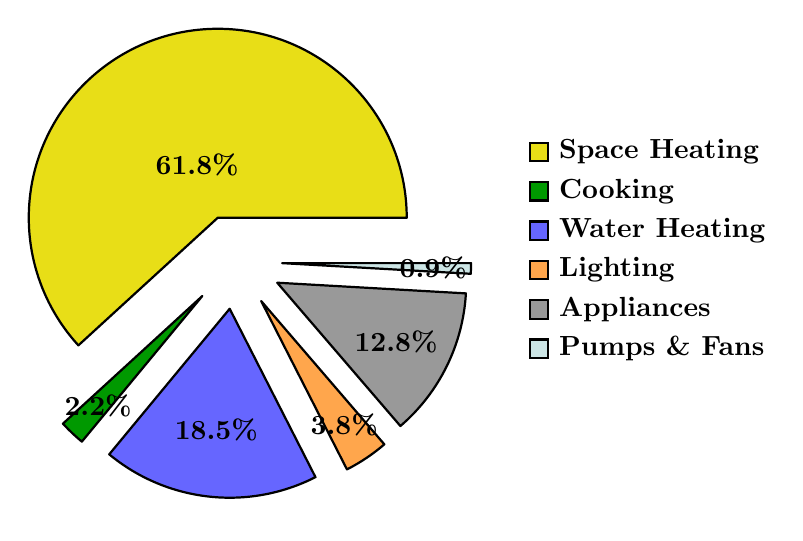
\begin{tikzpicture}
    \tikzstyle{every node}=[font={\bf}]
    \pie[   color = { yellow!90!black, green!60!black, blue!60,
        orange!70,
        gray!80,
        teal!20
    }, explode = 0.6, text=legend, radius=2.4]{61.8/Space Heating, 2.2/Cooking, 18.5/Water Heating, 3.8/Lighting, 12.8/Appliances,0.9/Pumps \& Fans}
    \end{tikzpicture}
    \caption{Ireland 2018 Energy Service Demands}
    \label{fig:Ireland2018ServiceDemands}
\end{figure}

Notably absent from Fig.\ref{fig:Ireland2018ServiceDemands}, is space cooling, which is accounted for in appliances. The Policy Oriented Tool for Energy and Climate Change Impact Assessment (POTEnCIA) project disaggregated Ireland's residential space cooling from appliances and have output expected space cooling energy consumption projections are shown in Fig.\ref{fig:Cooling}. 


Demand TIMESLICE 40  

\subsubsection{Space and Water Heating}
\label{LitR:Heating}

The demand for space and water heating is outlined in the previous section, and this section explains how water and space heating are achieved through technology and retrofits. While the demands are exogenous, the choice of technologies to at least satisfy the demand are endogenous and is captured in Equation \ref{Eq:Technology}.

\begin{equation} 
\begin{split}
Min \text{\euro} \sum_k VAR\_ACT_{k,i}(y)  \geq DM_i(y) 
\end{split}
\label{Eq:Technology}
\end{equation}

Where VAR\_ACT are the activity levels of end-use technology (k) for demand category (i) in year (y). DM is the exogenous demand per energy service per year. The cost of the technology used is minimised while also satisfying all constraints. 

All technologies are archetype specific and some technologies deliver both water and space heating, while other technologies can only deliver one type of heating, the list of available technologies is outlined in \ref{sec:appendixA4}. Retrofits are included as they satisfy the residential space heating demand, without consuming fuel. 
The Danish Energy Agency's Technology Data for Individual Heat Production dataset was input to TIM, this dataset is also used in the EU TIMES model, the dataset has high granularity and is continuously updated.

The number of main heating systems equals the number of dwellings, this assumption ignores any impact of secondary system heating. One expection in the rule is , which are only secondary heating systems. 


The base year heating energy consumption uses census data \cite{2016CensusIreland} from the CSO, dataset E1008 is used to obtain the fuel used in heating systems per archetype. The fuel usage is calibrated using the SEAI Energy Balance 2018. 

\subsubsection{Lighting, Appliances and Other}
\label{LitR:Lighting,Appliances}

Lighting, appliances, and pumps \& fans are all fueled by electricity, whereas cooking can be fueled by electricity, gas or LPG. As shown in Figure \ref{fig:Ireland2018ServiceDemands}, these energy services accounted for 20\% of energy consumption in 2018, however this share of consumption is expected to increase. 
Refrigeration, cloth washing, cloth drying, dish washing are under the appliances category and data is sourced from Topten \cite{Michel2016EnergyREPORT} and SEAI \cite{SustainableEnergyAuthorityofIreland2018EnergySector}. Cooking is also sourced from Eurostat's ``Energy consumption in households by type and end-used" excel datasheet and cross-checked with SEAI \cite{SustainableEnergyAuthorityofIreland2018EnergySector}  Appliances not included in this list are simply under the ``Other Appliances" category in TIM and these final values are cross-checked with POTEnCIA. Other Appliances include television, multimedia, and computer technology. Lighting and pumps \& fans are archetype specific energy services as the data is sourced from the BER database.  
Equation \ref{Eq:Technology} is also used, but unlike the heating energy service demands there is little or no choice in different technologies (k) for some of the demand categories (i), therefore, the model has no choice but to invest in a technology, however  cost and efficiency of each technology does determine the overall investment.

\subsubsection{User Constraints}
\label{LitR:Constraints}
The TIM model operates on the basis of perfect foresight, but
\textit{``in reality, the behaviours of consumers is not always economically rational"} \cite{Li2018IncorporatingModel} for this reason ``User Constraints" are applied in the residential sector to better reflect reality. The User Constraints applied to the residential sector include:
\begin{itemize}
 \item One Space and Water Heating System per household ( stoves excluded ) 
 \item Maximum 60\% of existing buildings to be retrofitted by 2030, and 95 \% by 2070. Maximum \% interpolated between 2030 and 2070. 
 \item A prerequisite electrical heat pump requirement is applied to each archetype, the percentage of dwellings which requires a shallow or deep retrofit before a heat pump can be installed (  B2 rating for heat pump ready dwelling ). Hybrid heat pumps are not included in this constraint. 
 \begin{table}[htbp]
  \centering
  \footnotesize
  \caption{Prerequisite Heat Pump Requirement}
    \begin{tabular}{r|rrr}
    \hline
    \multicolumn{1}{l}{Requirement} & \multicolumn{1}{l}{Apartment} & \multicolumn{1}{l}{Attached } & \multicolumn{1}{l}{Detached} \\ \hline
    No Retrofit  & 24.5 \%   & 14.3 \%   & 12 \% \\
    Shallow Retrofit  & 28.5 \%   & 34.7 \%  & 36.8 \% \\
    Deep Retrofit  & 47 \%   & 51 \%  & 51.2 \% \\
    \end{tabular}%
  \label{tab:HeatPumpConstraint}%
\end{table}%
 \item The natural gas grid is currently connected to 39\% of apartments, 52\% of attached dwellings and 12\% of detached dwellings. The total share of dwellings connected to the gas grid is an upper constraint to grow by 50\% for each archetype. 
\item Maximum fuel share in cooking for Gas and LPG is 40\% and 10\% respectively. Base year fuel share for Gas is 32\% and LPG is 1.5 \%.
\item Maximum 10\% solar input to dual fuel heating technology
\item Maximum 30\% gas input into gas hybrid heating pumps
\end{itemize}

 
While other constraints are applied in different sectors, which affect the residetinal sector and vice-versa, they are not listed in this paper. The growth constraints listed above are calculated using the following \cite{Loulou2016DocumentationI} : 
\begin{equation} 
\begin{split}
VAR\_CAP(t + 1) \leq (1 + G^{M(t+1)-M(t)}) \cdot VAR\_CAP(t)+K
\end{split}
\label{Eq:GrowthConstraint}
\end{equation}

Where $VAR\_CAP$ is the technology capacity in time period (t), G is the growth coefficient, defined as a new attribute of the technology and represents the maximum annual growth allowed for the capacity. The quantity $M(t+1)-M(t)$ is the number of years between the milestones of time periods t and t+1. The constant K is useful whenever the technology has no capacity initially, to allow the capacity to build over time. 

\section{Results}
\label{Results}

The newly developed TIM provides some valuable insights on each sector and the sectoral interconnections. The results outlined in this paper are based upon six scenarios. While TIM can only analysis the energy system, the other large source of GHG emissions is from agriculture, therefore some scenarios are labelled based on agriculture GHG reduction percentage and Energy System GHG reduction percentage, the six scenarios are:
\begin{itemize}
    \item \textbf{No Mitigation} Least cost solution, where no emissions constraints are imposed
    \item \textbf{With Additional Measures (WAM)} includes the implementation of Ireland’s CAP 2019.
    \item \textbf{A25E65} Agriculture GHG emissions reduce by 25\%, Energy system GHG emissions reduces by 65\% by 2030 compared to 2018.
    \item \textbf{A33E61} Agriculture GHGs reduces by 33\% and Energy system GHGs by 61\%
    \item \textbf{A40E57} Agriculture GHGs reduces by 33\% and Energy system GHGs by 61\%
    \item \textbf{A51E51} Equal GHG reduction share in of 51 \% in Agriculture and Energy Systems. 
\end{itemize}

While the first two scenarios do not comply with the Climate Action and Low Carbon Development (Amendment) Act 2021 target of an overall 51 \% GHG reduction in 2030 compared to 2018 or net-zero by 2050, however they do provide insights on the incremental steps required. The last four scenarios comply with 2030 and 2050 targets and offer insights about different trajectories to achieve those targets.  
Under CAP 2019 agriculture, GHG emission reduction is 10-15\% on the projected levels in 2030 relative to 2017. The higher agriculture ambition explored GHG reductions of 25-51\%. 

Figure \ref{fig:$CO_2$ Waterfall} provides an overview of  scenario affects on each sector in 2030, as the energy system ambition increases incrementally from left to right. 

\begin{figure}[!htbp]
 \centering
 \includegraphics[width=\textwidth]{Figures/CO2Waterfall.png}
 \caption{$CO_2$ Waterfall}
 \label{fig:$CO_2$ Waterfall}
\end{figure}

The share of sectoral $CO_2$ emissions is not evenly spread in 2018 and the optimal share of sectoral $CO_2$ reductions in 2030 is also unevenly distributed. In the A51E51 scenario, the optimal electricity annual emissions reduction is $7.1 MtCO_2$ in 2030, while transport currently emits the similiar $CO_2$ levels only reduces by $4.5 MtCO_2$. The residential sector reduces $CO_2$ emission by 63\% in A51E51 in 2030, electricity is 60 \% and transport is 38\%. Not only does Figure \ref{fig:$CO_2$ Waterfall} show the different optimal sectoral reductions, but also the ``low hanging fruit" in the large electricity reduction to the    ``high coconuts" in the step from A33E61 to A25E65, transport mitigates the majority of $CO_2$ emissions required. 

Zooming in and focusing on the fuel-mix within the residential sector gives further insights on the optimal pathways to achieve 2030 targets, Figure \ref{fig:ResFuel} shows this, with the base year stacked chart on the top row, the four climate bill compliant scenarios on rows 2-5 and the last two rows are non-compliant. 

\begin{figure}[!htbp]
 \centering
 \includegraphics[width=\textwidth]{Figures/RSD_Fuel2.png}
 \caption{Residential Fuel per scenario}
 \label{fig:ResFuel}
\end{figure}

In 2018, the residential sector had 124 PJ of primary energy that figure needs to decrease by 8-13 \% in 2030, to comply with climate targets. While Figure \ref{fig:$CO_2$ Waterfall} shows the large $CO_2$ reduction in electricity, this translates to a Figure \ref{fig:ResFuel} representing a large uptake of electricity in the residential sector within climate bill compliant scenarios. The large increase in ambient energy indicates the type of technology deployed in the residential sector, more on this in Figure XXX. The overall share of ambient heat increases from 1.4 \% in 2019 to between 13-26 \% in 2030. as a fuel  In climate bill compliant sceanrios peat and coal are completely phased out, while oil use decreases 90-93 \% by 2030. Gas energy increase by 34 \% in the A51E51 scenario, but remains relatively stable amoung other climate bill compliant sceanrios in 2030. 
By comparing compliant and noncompliant sceanrios, we can observe the favoured fuels and technologies, while also observing the incremental steps of emission reduction and overall cost change with each sceanrio. 

While Figure \ref{fig:ResFuel} shows the primary energy redcution required, it must be noted that retrofits are used to reduce the primary energy required ( reduced energy through behavioural change is not modelled ). Figure \ref{fig:Retrofits} shows both the number of retrofits per type and the energy savings for each of the four climate bill compliant scenarios. 

\begin{figure}[!htbp]
 \centering
 \includegraphics[width=\textwidth]{Figures/Retrofits.png}
 \caption{Retrofits by type per scenario}
 \label{fig:Retrofits}
\end{figure}
  
The number of retrofits required varies from 393,000 in A51E51 to 615,000 in A25E65, meaning between 23 - 36 \% of existing dwellings will require some form of retrofit.  
As mentioned in Table \ref{tab:HeatPumpConstraint}, the rollout of retrofits constraints the amount of heat pumps which can be installed, however, a certain share of existing dwellings and all new dwellings are heat pump ready, i.e B2 rating or above.  
\begin{figure}[!htbp]
 \centering
 \includegraphics[width=\textwidth]{Figures/HeatPumps.png}
 \caption{Heat Pump by type per scenario}
 \label{fig:HeatPump}
\end{figure}
 
Where SW is space and water heating, HC is space heating and space cooling and A-to-W represents air-to-water type heat pumps. The optimal number of heat pumps in each scenario ranges from 492,000 in A51E51 to 938,000 in A25E65, which equates to 23 - 45 \% of dwellings having a heat pump in 2030. Close to 45,000 air to water heat pumps are installed in apartments across all scenarios, as there are no retrofits in apartments, these heat pumps are installed in the existing B2 rating or above apartments or new apartments. The detached air-to-water heat pumps are the most prevalent across scenarios and maybe considered the low hanging fruit. 
 

The advantage of an energy system model is to observe the intersectoral connections. Figure \ref{fig:SectorFuel} presents a boxplot of the 2030 fuel consumption in four different sectors, under the four scenarios which comply with the 51 \% reduction.....
\begin{figure}[!htbp]
 \centering
 \includegraphics[width=\textwidth]{Figures/SectorFuel.png}
 \caption{Sector Fuel per scenario}
 \label{fig:SectorFuel}
\end{figure}



for further insights...


\begin{figure}[!htbp]
 \centering
 \includegraphics[width=\textwidth]{Figures/SectorCost.png}
 \caption{Sector Cost per scenario}
 \label{fig:SectorCost}
\end{figure}

Final Fuels share in each secotr Figure ....



\section{Discussion}
\label{Discussion}
5\% increase of residential energy in 2030 when internal temperatures are adjusted. 
Soft-linking with LEAP and PLEXOS
Gas is a faoured fuel from Fig \ref{fig:RESFuel} this provides insights on potential to decarbonise
%o	Discuss and interpret the results
%o	Focus on what added value the model brings
%o	Also include future development priorities here
%o	What can’t the model do? Where is it more suitable to use another model - Hannah Email
Retrofitting ``rebound" saving orangeuces energy other is more difficult to measure like improved physical and mental health. 
\subsection{Strengths}
\label{Dis:Strengths}

First iteration - of the model will need further development, DH, BEhavour, higher granularity, and spatial will be easily done with the dataset. 
%What does new model do that previous didn’t?
%TIM residential improvements - DH, HVO, Solar ( in progress ), better graps the cost and savings of retrofits and heat pumps, which can infrom MACC.Build with 2018 baseyear, not 2010 as previous versions had - this suits the 2030 target
%THe implications of net-zero
%Does new policy context require new modelling approach?
%Yes, do account for ongoing investments in climate mitigation opitions, the approach should provide higher granularity for likely pathways
%How does new modelling structure provide insights (give examples) in a way that previous model didn’t?
%Demands - 
%Improved more detailed Energy Service Demands
Detailed bottom-up model - using the 2018 base year ( in line with policy )
Updated technology
Combines energy system effects
Robust filteorange input data about housing stock

\subsection{Limitations}
\label{Dis:Limit}
BER Database - No PV Solar capacity, No Heat Pump ready, Large defaults, wall types check?)
Community Retrofits - Better Energy Communities is our national retrofit initiative with grant support of up to €28 million for 2021. We support new approaches to achieving energy efficiency in Irish communities.
%Discrepancies were investigated, and assumptions reviewed intuitively in order to achieve a good match.=
Consumers’ final investment decision can be
represented by “willingness-to-pay” curves – for
instance, around 10\% of owner-occupiers are willing
to invest in energy efficiency measures for a payback
time of 4 years, falling to 0\% for a payback time of
6 years for some consumer cohorts
Type of Tenure is ignoorange
BER aggeragateed
housing stock u-values
behaviour and occupancy
Area
expected energy consumption weakness of BER database as 
Actual energy consumption for dwellings of
similar or near identical construction may vary by up to 600%
depending on usage \cite{Sunikka-Blank2012BuildingConsumption}
\section{Conclusions}
\label{Conclusion}
This paper reports results on an ambitious mitigation target in the period to 2050 for the Irish energy system. The analysis has been performed using the Irish TIMES model
\textit{We stress the importance of differentiating between technical con-
straints and behavioural constraints in optimisation models. Including both conflates what is consideorange desirable under the economic welfare paradigm (i.e. cost-minimising decisions) with “realistic decisions”, complicating the interpretation of the results. Optimisation models are by design well suited to study cost-optimal behaviour, and running scenarios just with technical constraints facilitates the identification of areas where market barriers are more entrenched, and interventions to accelerate the uptake of low-carbon practices may be needed.} \cite{Astudillo2017CanModelb}
\section{Acknowledgements}
\label{sec:Acknowledgements}
Tomas %CAPACITY is funded under the Climate Action Modelling Group (CAMG) by DECC
% https://www.marei.ie/project/capacity/
CHIMERA is supported by a research grant from Science Foundation Ireland (SFI) and the National Natural Science Foundation of China (NSFC) under the SFI-NSFC Partnership Programme, grant no. 17/NSFC/5181 and
supported by MaREI, the SFI Research Centre for Energy, Climate, and Marine [Grant No: 12/RC/2302\_P2]


https://www.marei.ie/project/chimera/
\appendix

\section{}
\label{sec:appendix}
%% The Appendices part is started with the command \appendix;
%% appendix sections are then done as normal sections
\subsection{}
\label{sec:appendixA}
BER Database Filters
\begin{table}[htbp]
 \centering
 \footnotesize
 \caption{BER Filters}
 \begin{tabular}{ccc}
 \hline
 Filter Name & Data Removed & Reason \\
 \hline
 Ground Floor Area &  $<30m^2$ \& $>1000m^2$ & Consideorange erroneous \\
 Provisional Records & All & Higher Inaccuracies  \\
 Thermal Bridging Factor & $\leq0.15 W/m^2K$ & Outlier \\
 Declaorange Loss Factor & $>20kWh/day$ & Consideorange erroneous \\
 Living Area Percent & $<5\%$ \& $>90\%$ & Outlier \\
 Heat System Supply Heat Fraction & $>21\%$ & Outlier  \\
 Heat System Efficiency Adjustment Factor & $<0.7$ & Consideorange erroneous \\
 Main Space System Efficiency & $\leq19\%$ & Consideorange erroneous \\
Water System Efficiency Adjustment Factor & $<0.7$ & Consideorange erroneous\\
Main Water System Efficiency & $\leq19\%$ \& $>320\%$ & Consideorange erroneous \\
 \hline
 \end{tabular}%
 \label{BERFilters}%
\end{table}%

\subsection{}
\label{sec:appendixA2}
Age to BER Rating Correlation Index
\begin{sidewaystable}

\centering
 \footnotesize
 \caption{Apartment Age to BER Rating Correlation}
\begin{tabular}{l|lllllllll}
Year   & A      & B1     & B2     & B3     & C      & D      & E      & F      & G      \\ \hline
Before\_1919 & 0.0005 & 0.0021 & 0.0066 & 0.0139 & 0.0865 & 0.1618 & 0.1889 & 0.1447 & 0.3950 \\
1919-1945    & 0.0007 & 0.0075 & 0.0457 & 0.0689 & 0.1646 & 0.1775 & 0.1614 & 0.1100 & 0.2636 \\
1946-1960    & 0.0069 & 0.0146 & 0.0434 & 0.0553 & 0.1610 & 0.2085 & 0.1843 & 0.1139 & 0.2122 \\
1961-1970    & 0.0097 & 0.0173 & 0.0692 & 0.0736 & 0.2060 & 0.2208 & 0.1484 & 0.0957 & 0.1593 \\
1971-1980    & 0.0005 & 0.0014 & 0.0215 & 0.0305 & 0.2556 & 0.2809 & 0.2032 & 0.1009 & 0.1055 \\
1981-1990    & 0.0002 & 0.0003 & 0.0035 & 0.0249 & 0.2278 & 0.3223 & 0.2589 & 0.1036 & 0.0585 \\
1991-2000    & 0.0003 & 0.0016 & 0.0095 & 0.0293 & 0.3052 & 0.3728 & 0.2069 & 0.0546 & 0.0199 \\
2001-2010    & 0.0049 & 0.0310 & 0.0938 & 0.1504 & 0.4272 & 0.2033 & 0.0711 & 0.0140 & 0.0042 \\
Later\_2010  & 0.7996 & 0.0837 & 0.0713 & 0.0246 & 0.0140 & 0.0039 & 0.0019 & 0.0004 & 0.0005
\end{tabular}


\centering
 \footnotesize
 \caption{Attached Age to BER Rating Correlation}
\begin{tabular}{l|lllllllll}
Year         & A      & B1     & B2     & B3     & C      & D      & E      & F      & G      \\ \hline
Before\_1919 & 0.0021 & 0.0027 & 0.0091 & 0.0245 & 0.1239 & 0.1974 & 0.2109 & 0.1458 & 0.2837 \\
1919-1945    & 0.0019 & 0.0028 & 0.0102 & 0.0310 & 0.1835 & 0.2348 & 0.2046 & 0.1340 & 0.1973 \\
1946-1960    & 0.0023 & 0.0050 & 0.0130 & 0.0305 & 0.1991 & 0.2585 & 0.2309 & 0.1312 & 0.1295 \\
1961-1970    & 0.0032 & 0.0023 & 0.0100 & 0.0363 & 0.2757 & 0.3134 & 0.2021 & 0.0915 & 0.0654 \\
1971-1980    & 0.0022 & 0.0024 & 0.0069 & 0.0382 & 0.3452 & 0.3329 & 0.1738 & 0.0619 & 0.0365 \\
1981-1990    & 0.0010 & 0.0010 & 0.0069 & 0.0447 & 0.4263 & 0.3486 & 0.1198 & 0.0326 & 0.0190 \\
1991-2000    & 0.0011 & 0.0043 & 0.0084 & 0.0469 & 0.4833 & 0.3389 & 0.0835 & 0.0250 & 0.0087 \\
2001-2010    & 0.0045 & 0.0144 & 0.0438 & 0.1439 & 0.6330 & 0.1208 & 0.0303 & 0.0077 & 0.0016 \\
Later\_2010  & 0.9359 & 0.0391 & 0.0147 & 0.0064 & 0.0032 & 0.0006 & 0.0000 & 0.0000 & 0.0000
\end{tabular}


\centering
 \footnotesize
 \caption{Detached Age to BER Rating Correlation}
\begin{tabular}{l|lllllllll}
Detached     & A      & B1     & B2     & B3     & C      & D      & E      & F      & G      \\ \hline
Before\_1919 & 0.0035 & 0.0036 & 0.0078 & 0.0159 & 0.0912 & 0.1570 & 0.1791 & 0.1422 & 0.3996 \\
1919-1945    & 0.0044 & 0.0035 & 0.0083 & 0.0200 & 0.1059 & 0.1728 & 0.1762 & 0.1354 & 0.3734 \\
1946-1960    & 0.0055 & 0.0053 & 0.0127 & 0.0215 & 0.1298 & 0.2189 & 0.1928 & 0.1353 & 0.2782 \\
1961-1970    & 0.0061 & 0.0046 & 0.0118 & 0.0229 & 0.1770 & 0.2910 & 0.2240 & 0.1132 & 0.1494 \\
1971-1980    & 0.0034 & 0.0027 & 0.0090 & 0.0270 & 0.2663 & 0.3586 & 0.1942 & 0.0729 & 0.0660 \\
1981-1990    & 0.0027 & 0.0028 & 0.0091 & 0.0422 & 0.3641 & 0.3920 & 0.1285 & 0.0349 & 0.0237 \\
1991-2000    & 0.0019 & 0.0027 & 0.0152 & 0.0754 & 0.5372 & 0.2911 & 0.0519 & 0.0163 & 0.0082 \\
2001-2010    & 0.0081 & 0.0216 & 0.0643 & 0.1785 & 0.5903 & 0.1112 & 0.0172 & 0.0059 & 0.0029 \\
Later\_2010  & 0.8131 & 0.0868 & 0.0509 & 0.0295 & 0.0165 & 0.0029 & 0.0002 & 0.0002 & 0.0001
\end{tabular}
\end{sidewaystable}


%% If you have bibdatabase file and want bibtex to generate the
%% bibitems, please use
%%
\newpage

\subsection{}
\label{sec:appendixA3}
Depth of Retrofit defined by expected energy savings. The red cells are unfeasible, orange cells show deep retrofits and yellow represent shallow retrofits. 
%The model has two types of retrofitting options per archetype,  a shallow retrofit is when the primary energy ($kWh/m^2/yr$) is reduced by $ \leq 35 \%$, and deep retrofit is where the primary energy is reduced by $>35 \%$, a reduction of $ \> 75 \%$ is considered infeasible. The different between the pre-retrofit and post-retrofit primary energy determines the type of retrofit, as shown i

\begin{table}[htbp]
 \centering
 \footnotesize
 \caption{Energy Savings per BER rating}
 \begin{tabular}{|cl|llllllll}
\hline   
&  \multicolumn{8}{c}{Pre-Retrofit Rating}     \\ 
 & & G  & F & E & D  & C & B3  & B2  & B1 \\ \hline 
\multirow{8}{*}{\rotatebox[origin=c]{90}{Post-Retrofit Rating}} & A       & \cellcolor{red}83\% & \cellcolor{orange}73\% & \cellcolor{orange}67\% & \cellcolor{orange}57\% & \cellcolor{orange}38\%  & \cellcolor{orange}46\% & \cellcolor{yellow}35\% & \cellcolor{yellow}17\% \\
 & B1 & \cellcolor{red}79\% & \cellcolor{orange}68\%  & \cellcolor{orange}61\% & \cellcolor{orange}48\% & \cellcolor{yellow}25\%  & \cellcolor{yellow}35\% & \cellcolor{yellow}22\% &      \\
  & B2      & \cellcolor{orange}73\% & \cellcolor{orange}59\% & \cellcolor{orange}49\% & \cellcolor{yellow}33\% & \cellcolor{yellow}4\%   & \cellcolor{yellow}17\% &      &      \\
  & B3      & \cellcolor{orange}68\% & \cellcolor{orange}50\% & \cellcolor{orange}39\% & \cellcolor{yellow}19\% & \cellcolor{yellow}0\% &      &      &      \\
  & C       & \cellcolor{orange}72\% & \cellcolor{orange}57\% & \cellcolor{orange}47\% & \cellcolor{yellow}30\% &       &      &      &      \\
 & D       & \cellcolor{orange}60\% & \cellcolor{orange}\cellcolor{orange}38\% & \cellcolor{yellow}25\% &      &       &      &      &      \\
 & E       & \cellcolor{orange}47\% & \cellcolor{yellow}18\% &      &      &       &      &      &      \\
  & F       & \cellcolor{yellow}35\% &      &      &      &       &      &      &     

 \end{tabular}%
 \label{DepthofRetrofit}%
\end{table}

\newpage

\subsection{}
\label{sec:appendixA4}

List of water and space heating technologies available per archetype. The ``???" denotes either APT for Apartments, ATT for Attached, or DET for detached dwellings. 
\begin{table}[htbp]
  \centering
  \caption{Space and Water Heating Technologies}
  \resizebox{\textwidth}{!}{
 \begin{tabular}{cc|cc|cc|cc}
 \hline
  \multicolumn{2}{c|}{Technology} & \multicolumn{2}{c|}{Apartments} & \multicolumn{2}{c|}{Attached} & \multicolumn{2}{c}{Detached}  \\
 Name & Fuel/Description & Space  & Water  & Space  & Water   & Space  & Water \\
 \hline
  \multicolumn{8}{c}{Boiler or Stove}  \\
 \hline
 R-SH\_???\_KER\_N1 & Oil & \checkmark & \ding{55} & \checkmark & \ding{55} & \checkmark & \ding{55} \\
R-SW\_???\_KER\_N1 & Oil  & \checkmark & \checkmark & \checkmark & \checkmark & \checkmark & \checkmark \\
R-SW\_???\_KER\_N2 & Oil/Solar & \ding{55} & \ding{55} & \checkmark & \checkmark & \checkmark & \checkmark \\
R-SW\_???\_KER\_N3 & Oil/Biomass & \ding{55} & \ding{55} & \checkmark & \checkmark & \checkmark & \checkmark \\
 R-SH\_???\_GAS\_N1 & Gas  & \checkmark & \ding{55} & \checkmark & \ding{55} & \checkmark & \ding{55} \\
R-SW\_???\_GAS\_N1 & Gas  & \checkmark & \checkmark & \checkmark & \checkmark & \checkmark & \checkmark \\
R-SW\_???\_GAS\_N2 & Gas/Solar  & \ding{55} & \ding{55} & \checkmark & \checkmark & \checkmark & \checkmark \\
R-SW\_???\_GAS\_N3 & Gas/Biomass  & \ding{55} & \ding{55} & \checkmark & \checkmark & \checkmark & \checkmark \\
 R-SH\_???\_LPG\_N1 & LPG  & \checkmark & \ding{55} & \checkmark & \ding{55} & \checkmark & \ding{55} \\
R-SW\_???\_LPG\_N1 & LPG  & \checkmark & \checkmark & \checkmark & \checkmark & \checkmark & \checkmark \\
 R-SH\_???\_WOO\_N1 & Biomass  & \checkmark & \ding{55} & \checkmark & \ding{55} & \checkmark & \ding{55} \\
R-SW\_???\_WOO\_N1 & Biomass  & \checkmark & \checkmark & \checkmark & \checkmark & \checkmark & \checkmark \\
R-SH\_???\_FPL\_N1 & Stove & \ding{55} & \ding{55} & \checkmark & \ding{55} & \checkmark & \ding{55} \\
R-SW\_???\_FPL\_N1 & Stove & \ding{55} & \ding{55} & \checkmark & \checkmark & \checkmark & \checkmark\\
R-SH\_???\_HVO\_N1 & HVO  & \ding{55} & \ding{55} & \checkmark & \ding{55} & \checkmark & \ding{55} \\
R-SW\_???\_HVO\_N1 & HVO  & \ding{55} & \ding{55} & \checkmark & \checkmark & \checkmark & \checkmark \\
 \hline
  \multicolumn{8}{c}{Electrical}  \\
 \hline
R-SH\_???\_ELC\_N1 & Resistance Heater & \checkmark & \ding{55} & \checkmark & \ding{55} & \checkmark & \ding{55} \\
 \hline
  \multicolumn{8}{c}{Electrical Heat Pumps}  \\
 \hline
R-SH\_???\_ELC\_HPN1 & A-to-A  & \ding{55} & \ding{55} & \ding{55} & \ding{55} & \ding{55} & \ding{55} \\
R-HC\_???\_ELC\_HPN1 & A-to-A  & \ding{55} & \ding{55} & \ding{55} & \ding{55} & \ding{55} & \ding{55} \\
R-SH\_???\_ELC\_HPN2 & A-to-W & \checkmark & \ding{55} & \checkmark & \ding{55} & \checkmark & \ding{55} \\
R-SW\_???\_ELC\_HPN1 & A-to-W & \checkmark & \checkmark & \checkmark & \checkmark & \checkmark & \checkmark \\
R-SW\_???\_ELC\_HPN2 & A-to-W  w/Solar & \ding{55} & \ding{55} & \checkmark & \checkmark & \checkmark & \checkmark \\
R-SH\_???\_ELC\_HPN3 & G-to-W  & \ding{55} & \ding{55} & \checkmark & \ding{55} & \checkmark & \ding{55}\\
R-HC\_???\_ELC\_HPN2 & G-to-W & \checkmark& \ding{55} & \checkmark & \ding{55} & \checkmark & \ding{55}\\
 \hline
  \multicolumn{8}{c}{Gas and Hybrid Heat Pumps}  \\
 \hline
 R-SW\_???\_GAS\_HPN1 & Gas Absorption & \checkmark & \checkmark & \checkmark & \checkmark & \checkmark & \checkmark\\
 R-SW\_???\_GAS\_HPN2 & Gas Engine & \checkmark & \checkmark & \checkmark & \checkmark & \checkmark & \checkmark\\
 R-SW\_???\_GAS\_HHPN1 & Gas Hybrid & \checkmark & \checkmark & \checkmark & \checkmark & \checkmark & \checkmark\\
  \hline
  \multicolumn{8}{c}{District Heating}  \\
 \hline
R-SW\_???\_HET\_N1 & Centralized & \checkmark & \checkmark & \checkmark & \checkmark & \checkmark & \checkmark\\
R-SW\_???\_HET\_N2 & Decentralized & \checkmark & \checkmark & \checkmark & \checkmark & \checkmark & \checkmark \\
  \hline
  \multicolumn{8}{c}{Water Heat Only}  \\
 \hline
 R-WH\_???\_ELC\_N1 & Resistance Heater  & \ding{55} & \checkmark & \ding{55} & \checkmark & \ding{55} & \checkmark \\
 R-WH\_???\_ELC\_N2 & Solar Thermal  & \ding{55} & \checkmark & \ding{55} & \checkmark & \ding{55} & \checkmark \\
   \hline
  \multicolumn{8}{c}{Retrofits}  \\
 \hline
 R-FTFT-???\_Shallow & Shallow Retrofit & \checkmark & \ding{55} & \checkmark & \ding{55} & \checkmark & \ding{55} \\
 R-FTFT-???\_Deep & Deep Retrofit & \checkmark & \ding{55} & \checkmark & \ding{55} & \checkmark & \ding{55} \\
 \end{tabular}%
 }
 \label{HeatingTech}%
\end{table}

\newpage

\printbibliography


%% else use the following coding to input the bibitems directly in the
%% TeX file.

%%\begin{thebibliography}{00}


% %% \bibitem[Author(year)]{label}
% %% Text of bibliographic item

% \bibitem[ ()]{}

% \end{thebibliography}
\end{document}
\endinput
%%
%% End of file `elsarticle-template-harv.tex'.
